% !TeX spellcheck = en_US
\addscenariosection{1}{Clash/Alliance Scenario}{Astral Run}{\images/astral.png}

\begin{multicols*}{2}

\textbf{Author:} LAAMAKALA

\textit{Every move could be your last. Every gate a gamble. Glory belongs to the bold}

\subsection*{\MakeUppercase{Scenario Length}}
This Scenario plays out over 16 Rounds

\subsection*{\MakeUppercase{Player Setup}}
\textbf{Player Count:} 2 -- 6

\textbf{Starting Resources:} 14 \svg{gold}, 4 \svg{building_materials}, 1 \svg{valuables}

\textbf{Starting Income:} 10 \svg{gold}, 0 \svg{building_materials}, 0 \svg{valuables}

\textbf{Starting Units:}

\begin{itemize}
  \item A Pack \bronze\ Units of the player's choosing
\end{itemize}

\textbf{Town Buildings:}
\begin{itemize}
  \item \bronze\ Dwelling
  \item Each player may build the \svg{building_special_tent} building with a discount of 4 \svg{gold} and 2 \svg{building_materials}.
\end{itemize}

\subsection*{\MakeUppercase{Map Setup}}
Take the following Map Tiles ($P$ stands for the number of players) and arrange them as shown in the Scenario map layout:

\begin{itemize}
  \item P × Starting (I) Map Tile
  \item 2P × Far (II-III) Map Tiles
  \item P × Near (IV-V) Map Tile
  \item 6 × Near (IV-V) Map Tiles with Obelisk
  \item 1 × Center (VI-VII) Map Tile
\end{itemize}

\subsection*{\MakeUppercase{Victory Conditions}}
The game ends at the end of the Round when any of these conditions are met:

\begin{itemize}
  \item One player has defeated each other player's Main Heroes once - \textit{That player wins the game immediately.}
  \item One player controls the Center VII Field for 3 consecutive Rounds- \textit{That player wins the game immediately.}
  \item At the end of Round 16.
\end{itemize}

\subsection*{\MakeUppercase{Victory Points}}
If no player has achieved an immediate victory, the player with the most Victory Points (VP) wins.
In addition to the Tournament Book's ``Scoring Victory Points'' section, players get VPs for:

\begin{itemize}
  \item 5 VP for first player Flagging Center VII Field.
  \item 1 VP for every flagged Mine and Settlement on Near and Center Tiles.
  \item Removed Artifacts also count towards VPs.
\end{itemize}

\subsection*{\MakeUppercase{Timed Events}}

\begin{itemize}
  \item[\textbf{\nth{1}}] \textbf{Round:} All Heroes gain +1 \svgeven{movement}.
  \item[\textbf{\nth{4}}] \textbf{Round:} Remove all Black Cubes.
  \item[\textbf{\nth{6}}] \textbf{Round:} Player(s) whose Main Hero has the least \svg{experience}, Search (2) \svg{artifact}.
  \item[\textbf{\nth{9}}] \textbf{Round:} Remove all Black Cubes.
  \item[\textbf{\nth{10}}] \textbf{Round:} Player(s) whose Main Hero has the least \svg{experience}, roll 2 \svg{resource}.
  \item[\textbf{\nth{12}}] \textbf{Round:} Remove all Black Cubes.
  \item[\textbf{\nth{13}}] \textbf{Round:} All Heroes gain +1 \svgeven{movement}.
\end{itemize}

\end{multicols*}

\begin{multicols}{2}

\subsection*{\MakeUppercase{Additional Rules}}
\begin{itemize}
  \item \textbf{Sanctuary:} Gain 1 \svg{morale_positive} token and draw 1 Card from your Deck. \textit{Visitable once per Faction}.
  \item \textbf{Obelisk:} Guarded by Level VI Neutrals. Roll one \svg{resource} and draw one Card. \textit{Visitable once per Faction}.
  \item Each blocked Field adjacent to an Obelisk is a two-way Astral Gate, which only becomes active after that Obelisk has been visited.
  \item An Astral Gate cannot be entered from a different Map Tile. When a Hero enters an Astral Gate, they are teleported to another random activated Astral Gate on the Map and arrive on an adjacent Field.
  \item Instead of teleporting randomly, a player may spend 1 \svg{morale_positive} to choose the destination Astral Gate.
  \item Gain 1 \svg{experience} after a Combat against an enemy Main Hero.
  \item A defeated Main Hero may Empower one Defense Statistic Card from their M\&M Deck.
  \item Players do not have to pay \svg{gold} after losing a Combat against another player.
\end{itemize}

\end{multicols}

\begin{tikzpicture}[overlay, remember picture]
  \node[yshift=-8em] at (current page.center) {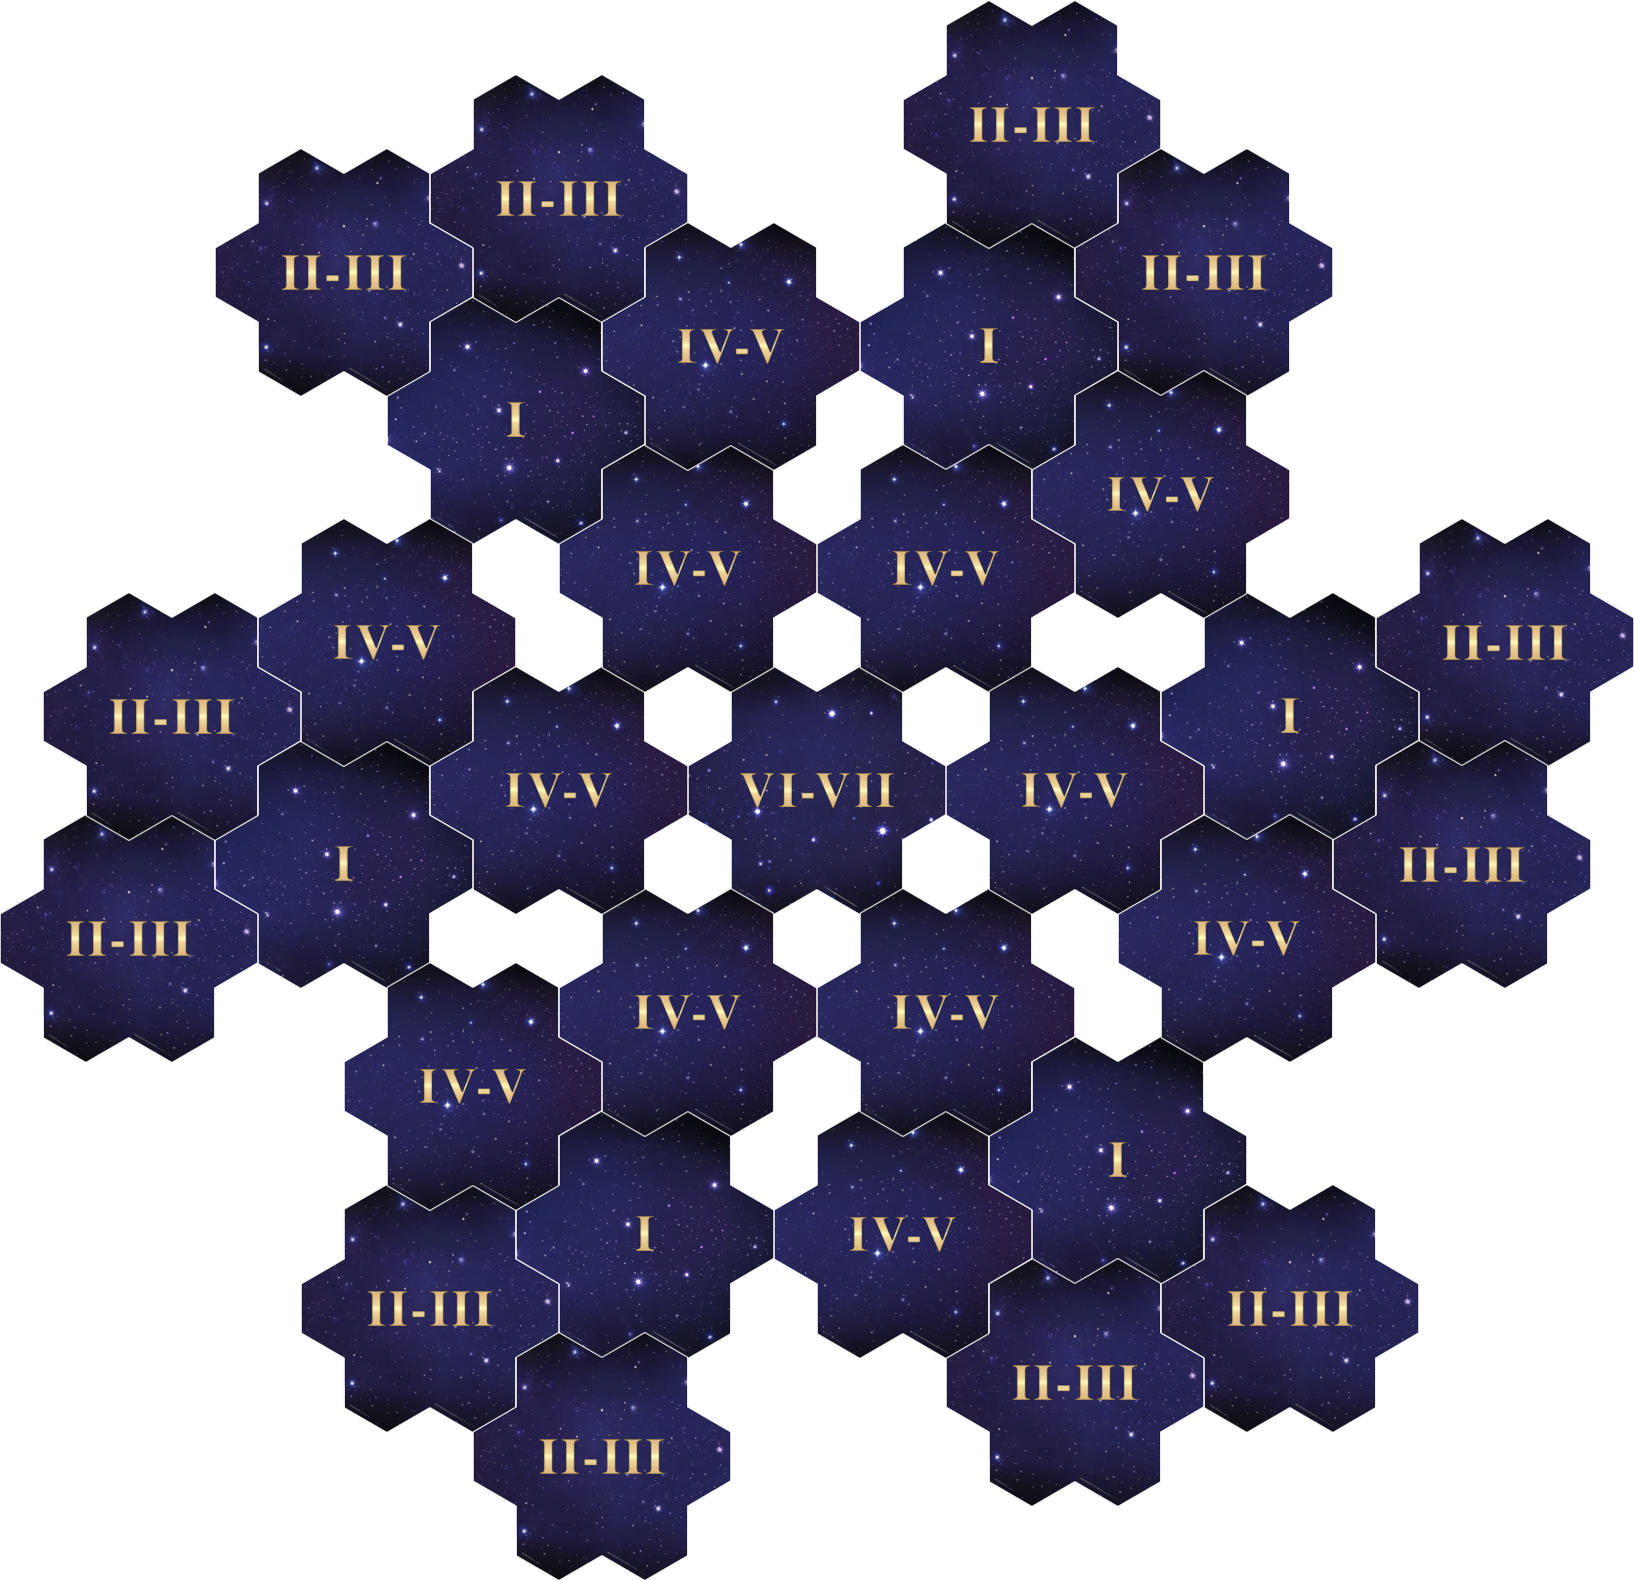
\includegraphics[width=0.9\linewidth]{\maps/astral_run.png}};
\end{tikzpicture}
